% 3.4.2 Contenedores e integración y entrega continuas (T6).
% Memoria: docker stats --no-stream, sin carga de usuarios.

\subsubsection{Contenedores e integración y entrega continuas}
\label{sec:ob3_cicd}

Un único archivo de Docker Compose levanta los contenedores del diseño (Tabla~\ref{tab:ob3_contenedores}). La memoria medida ronda los 0,6 GB, dentro de lo estimado (Tabla~\ref{tab:ob2_riesgos}).

\begingroup
\fontsize{9}{11}\selectfont
\renewcommand{\arraystretch}{1.2}
\setlength{\LTpre}{0pt}\setlength{\LTpost}{6pt}
\setlength{\tabcolsep}{4pt}
\begin{xltabular}{\linewidth}{|>{\raggedright\arraybackslash}p{2.8cm}|>{\raggedright\arraybackslash}X|c|c|}
\caption{Contenedores en producción y memoria medida}
\label{tab:ob3_contenedores} \\
\hline
\textbf{Contenedor} & \textbf{Función} & \textbf{Uso (MB)} & \textbf{Límite (MB)} \\ \hline
\endfirsthead
\hline
\textbf{Contenedor} & \textbf{Función} & \textbf{Uso (MB)} & \textbf{Límite (MB)} \\ \hline
\endhead
Proxy (Caddy) & Única entrada pública; HTTPS & 19 & 128 \\ \hline
Aplicación web & Interfaz de la secretaria, el odontólogo y el director & 6 & 64 \\ \hline
API & Reglas del negocio y única escritura en la base de datos & 466 & 1\,024 \\ \hline
Agente & Webhook de WhatsApp y conversación & 44 & 256 \\ \hline
Base de datos & PostgreSQL 16, sin puerto expuesto & 59 & 1\,024 \\ \hline
\textbf{Total} & & \textbf{594} & \textbf{2\,496} \\ \hline
\end{xltabular}
\endgroup

\textit{[Respaldo: contenedor, frecuencia, destino y prueba de restauración.]}

Cada repositorio publica sus cambios con el mismo flujo de GitHub Actions (Figura~\ref{fig:ob3_cicd}): pruebas, imagen en GitHub Container Registry y despliegue por SSH. Si una prueba falla, no se despliega. Antes de actualizar la API se respalda la base de datos, y el despliegue espera a que el contenedor responda como sano; para volver atrás se despliega la etiqueta anterior.

\begin{figure}[H]
\centering
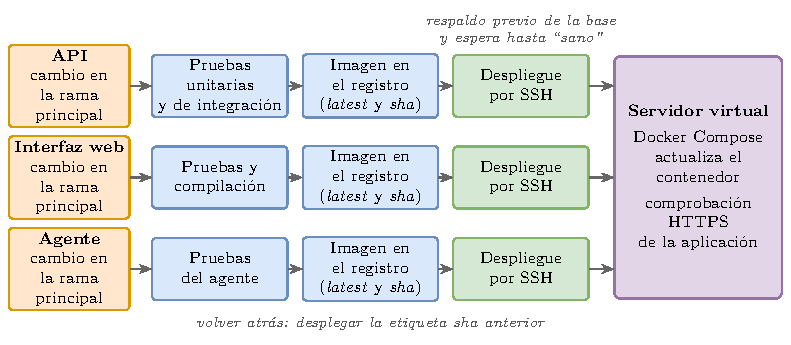
\includegraphics[width=\linewidth]{img/Objetivo3/Ob3_CICD.pdf}
\caption{Flujo de integración y entrega continuas}
\label{fig:ob3_cicd}
\end{figure}
